\chapter{Projekt}
\thispagestyle{chapterBeginStyle}
W danym rodziale opisana została aplikacja pod względem technicznym. 

\section{Opis systemu}
Tworzenie aplikacji internetowej to skomplikowany proces, który może przysporzyć wiele problemów w przyszłości. Pierwszym problemem jest utrzymanie istniejącego kodu, to znaczy kontrolowanie stanu aplikacji i naprawianie pojawiających się błędów, związanych z pierwotną implementacją. Drugim problemem jest możliwość rozwoju aplikacji, w momencie w którym aplikacja przynosi zyski i sprawdza się w kontakcie z użytkownikiem, oczywistym podejściem jest rozbudowa aplikacji. W tym celu podczas planowania implementacji trzeba zastanowić się nad odpowiednim podejściem. W tym celu powstały wzorce projektowe, które pomagają programistom uporać się z różnymi problemami w sposób zorganizowany i zoptymalizowany, ułatwiają rozwiązywanie błędów podczas implementacji oraz zwiększają czytelność kodu.

\section{Wzorzec architektoniczny Model-View-Controller}
System zbudowany został w oparciu o model MVC, czyli Model-View-Controller.
Jest to podejście architektoniczne, które dzieli aplikację na trzy główne komponenty.
Model, odpowiedzialny za dostęp i przechowywanie danych. View, czyli widok odpowiada za interfejs użytkownika, jak dane są przedstawiane i odbierane. Controller zajmuje się logiką biznesową komunikując się z modelem i widokiem. Widok dostarcza informacje od klienta, które obsługiwane są przez Controller i odpowiednie zmiany wprowadzane są do modelu. \cite{6827095}

\begin{figure}[h]

	\centering
		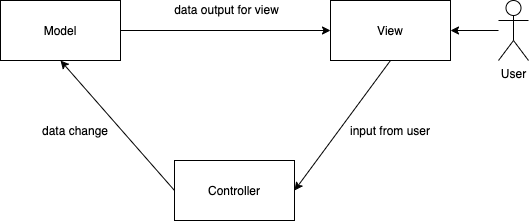
\includegraphics[width=0.90\textwidth]{mvc-diagram}		
		\caption{Komunikacja pomiędzy komponentami we wzorcu MVC }
\end{figure}

Zalety korzystania z wzorca MVC to lepsza przejrzystość kodu, skalowalność i utrzymanie. W
momencie wystąpienia błędu, może zostać obarczona odpowiedzialnością jedna z trzech części
systemu, więc optymalizuje to znacząco proces szukania miejsca, w którym dany błąd
występuje.  
\clearpage
\section{Wymagania funkcjonalne i niefunkcjonalne}
\paragraph{Wymagania funkcjonalne}
\begin{enumerate}
	\item Przegląd listy użytkowników
	\item Przegląd listy zadań 
	\item Tworzenie, edytowanie, usuwanie zadań
	\item Korzystanie z Tablicy Kanban w celu raportowania postępów w zadaniach
	\item Wyświetlanie Statystyk projektu w postaci wykresów
	\item Podstawowa autentykacja użytkownika
	\item Wyświetlanie szczegółów związanych z danym zadaniem. Szczegółowe parametry zadania to:
	\begin{enumerate}[leftmargin=3em]
		\item nazwa,
		\item data do zakończenia zadania,
		\item użytkownik przypisany do zadania, 
		\item kolumna w której aktualnie znajduje się dane zadanie,
		\item opis zadania
		\item sekcja komentarzy
		\item nazwa użytkownika tworzącego zadanie
	\end{enumerate}
\end{enumerate}
\paragraph{Wymagania funkcjonalne dodatkowe dla administratora}

		\begin{enumerate} 
		\item Tworzenie, aktywacja kont użytkowników, dostęp do większej ilości danych w porównaniu do użytkownika
		\item Ustawienie czasu po jakim czyszczona jest historia czynności związanych z zadaniami
		\item Konfiguracja tablicy:
	\begin{enumerate}[leftmargin=3em]
			\item określenie nazwy tablicy i kolumn
			\item określenie liczby kolumn, 
			\item wybranie domyślnej kolumny (na którą wprowadzane będą nowe zadania)
			\item wybranie końcowej kolumny ( która automatycznie zmienia status zadania na skończony) –  opcjonalne
		\end{enumerate}

\end{enumerate}

\paragraph{Wymagania niefunkcjonalne}
\begin{enumerate}
	\item możliwość użytkowania systemu po godzinnym szkoleniu
	\item komunikacja z bazą dancyh nie dłuższa niż 100ms na każde zapytanie 
	\item aplikacja responsywna, wymagania funkcjonalne możliwe były do wykonania na urządzeniu mobilnym
\end{enumerate}

\clearpage
\section{Diagram pakietów}

Pakiety podzielone są na elementy serwera i aplikacji webowej, przedstawione zostały na diagramie ~\ref{pakiet}.
\paragraph{Serwer }
\paragraph{Repository}
posiada charakterystyczne dla wzorca architektonicznego Spring Data klasy z annotacją @Repository. Są to klasy, które udostępniają gotowe metody do
wyciągania potrzebnych danych z bazy

\paragraph{domain}

definiuje model danych. Są to Tabele i ich wszystkie atrybuty przepisane na klasę z której korzystają klasy z pakietu repository
\paragraph{config}
jak sama nazwa wskazuje posiada wszystkie klasy związane z konfiguracją serwera poczynając od sposobu formatowania dat, wyboru domyślnego języka strony, czy też konfigurację dostępu użytkowników do potrzebnych interfejsów.
\paragraph{service}  to grupa klas z annotacją @Service odpowiedzialnych za wykonywanie logiki związanej z modyfikacją i odpowiednim zapisywaniem danych. Korzysta z pakietu repository, a sam wykorzystywany jest w pakiecie rest.
\paragraph{rest}  jest odpowiedzialny za transfer danych sposobem REST, czyli udostępnia  metody korzystające z serwisów na podane URI. Przykładowo aplikacja webowa wysyła na serwer zapytanie HTTP POST na URI
\textit{www.taskManager.com/task}. Serwer odczytuje zapytanie i przygotowywuje odpowiedź, w tym celu odpowiednia klasa z pakietu rest mapuje podane zapytanie do odpowiedniej metody, która wykonuje akurat w tym przykładzie zapisanie zadania do bazy danych i zwraca zwrotną wiadomość ~\ref{przykładowa metoda controllera}.

\paragraph{security} zawiera klasy odpowiedzialne za autentykację połączenia, zanim jakiekolwiek zapytanie trafi do metod z pakietu rest, najpierw serwer oczekuje na odpowiedź ze strony klienta odnośnie sukcesu autoryzacji i pozwoleń jakie zalogowany użytkownik posiada.

\begin{lstlisting} [ caption=Uproszczona metoda kontrolera z pakietu rest, captionpos=b, label={przykładowa metoda controllera}]
	
	@PostMapping("/task")
	public ResponseEntity<Task> createTask(@Valid @RequestBody TaskDTO taskDTO){
		if (taskDTO.getId() != null) {
			(...)
		}
		return ResponseEntity
		.headers(HeaderUtil.createAlert(applicationName))
		.body(task);
	}
	
\end{lstlisting}

\paragraph{aplikacja webowa}
\paragraph{config, model i service} to pakiety o tych samych właściwościach co w serwerze. Warto zauważyć, że model zapisany po stronie klienta może być ograniczony do atrybutów potrzebych jedynie do odpowiedniego wyświetlenia interfejsu dla użytkownika. 
\paragraph{user-view} posiada wszystkie komponenty widoków dostępne dla użytkownika i administratora, są to główne widoki aplikacji, takie jak tablica, statystyki, lista zadań i tym podobne.
\paragraph{admin} posiada komponenty dostępne tylko dla administratora i wszelką logikę związaną z konfiguracją nowych użytkowników.
\paragraph{shared} jest to pakiet, na który składają się wszystkie wspólne dla wszystkich innych klas komponenty, czyli bloki wyświetlające błędy, responsywna lista, nagłówek strony, stopka strony. 

 Poniżej znajduje się diagram pakietów projektu wygenerowany przez narzędzie do rysowania diagramów diagrams.net \cite{diagrams}
\begin{figure}[h]
	
	\centering
	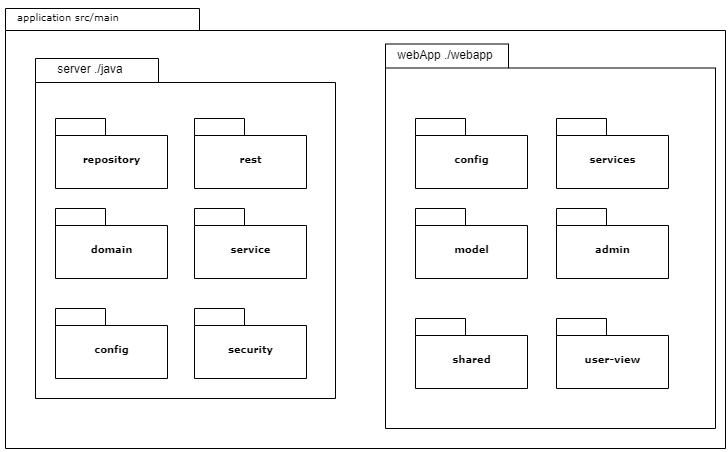
\includegraphics[width=0.90\textwidth]{pakiety}		
	\caption{Diagram pakietów z których złożona jest cała aplikacja }
	\label{pakiet}
\end{figure}


\section{Komunikacja klient - serwer}
Zbiór założeń, który definiuje komunikację pomiędzy systemami nazywamy API (z angielskiego Application Programming Interface, czyli interfejs programowania aplikacji).  Komunikacja odbywa sie za pomocą protokołów HTTP. Protokół HTTP jest to zestaw reguł odnośnie komunikacji polegający na wysyłaniu żądania i oczekiwaniu na odpowiedź. Klient wysyła zapytania, oczekuje na odpowiedź, a serwer oczekuje na zapytania odsyłając odpowiedź \cite{rfc7230}.
\newline
Protokół ten składa się z:
\begin{itemize}
	\item Metoda protokołu i wersja
	\item Nagłówka (z ang. header), który posiada wszystkie potrzebne informacje na temat połączenia
	\item Treści wiadomości (z ang. body)
	\item wiadomość zwrotna zawsze posiada status odpowiedzi w postaci kodu i wiadomości (naprzykład 200 OK)
\end{itemize}
Metody protokołu pozwalają rozróżnić rodzaj wiadomości. W aplikacji używana są metody:
\begin{itemize}
	\item POST  - wiadomość przychodząca od klienta, zazwyczaj używany do stworzenia obiektu na bazie danych
	\item GET - zapytanie o pobór danych za pomocą wskazanej ścieżki
	może to być lista obiektów z bazy danych czy też jeden specyficzny obiekt, którego identyfikator zawarty jest w ścieżce ( /api/task/1)
	\item PUT - jest to pokrewna metoda do POST, lecz używana do aktualizowania istniejących danych zamiast wprowadzania nowych
	\item DELETE - metoda służy do usuwania zasobów z bazy danych
\end{itemize}
Klient do komunikacji używa klas zaimplementowanych w pakiecie \textit{services}. Składają się one z prostych metod, które potrzebują jedynie odpowiednią ścieżkę, odpowiednią metodę HTTP i oczekiwany typ danych.
Klasy w pakiecie \textit{rest} serwera udostępniają metody na poszczególne ścieżki, w których zastosowana jest logika i zwracane zostają odpowiednie dane, wiadomość OK ze statusem 200 [~\ref{przykładowa metoda controllera}].

\section{Baza danych}

\subsection{Projekt}
Sekcja ta w pełni skupiona jest na budowie bazy danych. Jako baza danych wykorzystana została baza dystrubucji MySql jako że jest to jedna z relacyjnych baz danych ogólnodostępnych. MySql cechuje się skalowalnością i przede wszystkim ochroną danych. Wraz z możliwościami rozwoju danej aplikacji, postawiono na uniwersalną bazę danych, którą bez problemu można rozbudować i skomplikować.
W celu kontroli wersji projektu bazy danych do serwera podpięta jest biblioteka zwana Liquibase, która przechowuje wszystkie skrypty związane z tworzeniem bazy danych, modyfikacją tabel lub danych w formacie XML. Liquibase pomaga wprowadzać zmiany na istniejącej bazie danych przy zachowaniu poprzedniego stanu, zostawiając po udanej modyfikacji historię zmian. 
\begin{figure}[h]
	\centering
	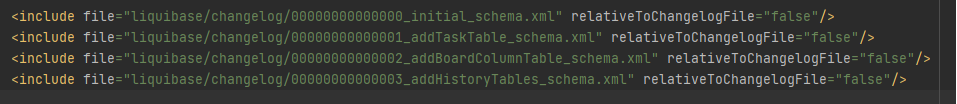
\includegraphics[width=0.90\textwidth]{liqubase}		
	\caption{Lista plików tworzących bazę danych }
	\label{listaplikow}
\end{figure}
Bilbioteka liquibase dodaje dwie tabele \ref{liqutable}, które dotyczą powyższej listy plików \ref{listaplikow}. Tabela zapisuje nazwę pliku i jej sumę kontrolną, więc zapobiega to zmianom na plikach inicjalizujących bazę danych. Trzeba stworzyć następny plik i pozsotawić po sobie ślad. Jest to bardzo pomocna rzecz, służy jako kontrola wersji bazy danych, aby w każdym momencie można było wrócić do wcześniejszych struktur bazy danych.
\begin{figure}[h]
	\centering
	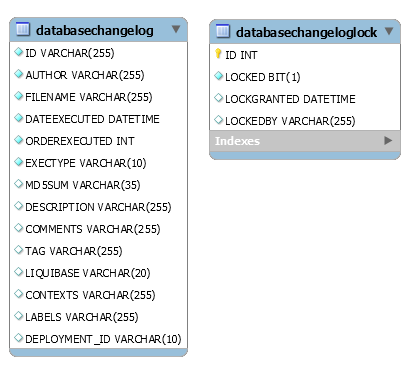
\includegraphics[width=0.50\textwidth]{liquibasetables}
	\caption{ Tabele kontroli wersji}
	\label{liqutable}
\end{figure}
Pierwszym rodzajem danych jest \textit{Tablica} ( board), która przetrzymuje informacje o tablicy. Kolejnym typem jest  \textit{Kolumna} ( column). Ważnym typem danych jest  \textit{Użytkownik}  (user), to jedna z najbardziej skomplikowanych tabel w całej bazie. Tabela z użytkownikami przetrzmuje informacje dotyczące korzystania z aplikacji i te  pozwalające autoryzować sesję po stronie klienta. Posiada również relacje z tabelą authority, która znowu odpowiedzialna jest za nadawnianie odpowiednich uprawnień do korzystania z aplikacji. Ostatnimi  danymi są \textit{Zadanie} (task) i \textit{Komentarz} (comment). Wszystkie relacje zostały przedstawione na diagramie ~\ref{projektdb}.
Oprócz głównych tabel do bazy danych dodane zostały również trzy nierelacyjne tabele, które audytują trzy zachowania, przeciąganie zadania z jednej kolumny na drugą (task\_drag\_drop), przetrzymywanie daty skończenia (task\_completed) i daty przypięcia zadania do użytkownika (task\_assignment) \ref{nierel}.

\begin{figure}[h]
	\centering
	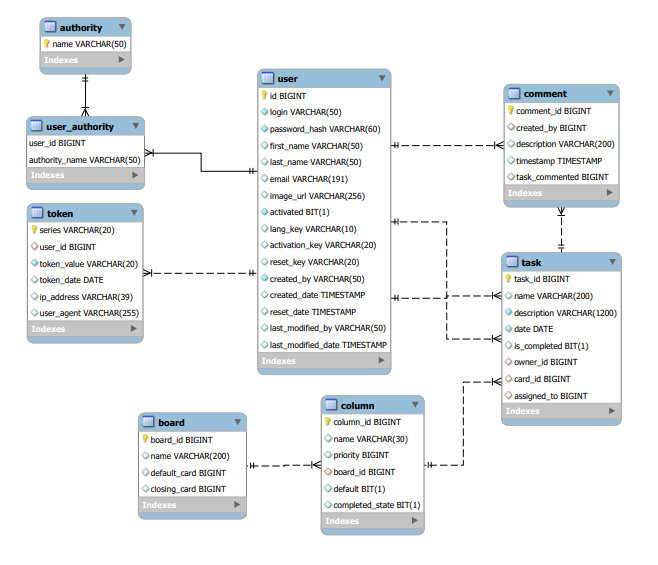
\includegraphics[width=0.90\textwidth]{diagram-bazy}

	\caption{ Diagram bazy danych}
		\label{projektdb}
\end{figure}


\begin{figure}[h]
	\centering
	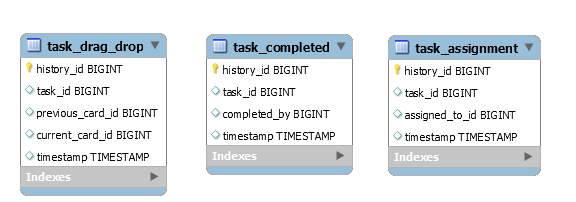
\includegraphics[]{nierelacyjne}

	\caption{ Nierelacyjne tabele odpowiedzialne za przetrzymywanie danych potrzebnych do statystyk }
	\label{nierel}
\end{figure}
\clearpage
\subsection{Normalizacja}
Schemat bazy danych stworzony może zostać na wiele, niekoniecznie dobrych sposobów. Normalizacja to czynność, która prowadzi do zoptymalizowania sposobu przetrzymywania danych]. Polega ona na odpowiednich zmianach na tabelach i relacjach, zgodnie z pewnym zbiorem zasad, w celu wyeliminowania niepotrzebnych relacji oraz redundancji danych. Pierwsze trzy zbiory reguł normalizacyjnych nazwane i zdefiniowane zostały przez Edgara Franka Codda. Jest to pierwsza postać normalna (1NF), druga postać normalna (2NF) i trzecia postać normalna (3NF). Zbiory te mają ze sobą pewną zależność. Pierwsza postać normalna jest podzbiorem reguł drugiej postaci normalnej, a druga postać normalna jest podzbiorem trzeciej postaci normalnej. Istnieje więcej postaci normalnych, lecz projekt bazy danych opisywanej aplikacji poddany został normalizacji do 3NF. \cite{db}

\subsubsection{Pierwsza postać normalna}
	\begin{definition}
 		Relacja jest w pierwszej postaci normalnej jeśli każda krotka posiada dokładnie jedną wartość dla danego atrybutu oraz nie istnieją powtarzające się krotki.
	\end{definition}
Wszystkie tabele spełniają pierwszą postać normalną. Każda tabela dzieli dane na kolumny o atomowych wartościach. Nigdzie nie występują krotki posiadające listę wartości. Wartości typu imię i nazwisko użytkownika zostały podzielone na osobne kolumny. Krotki nie powtarzają się, ponieważ każda tabela posiada klucz główny.
	
\subsubsection{Druga  postać normalna}
	\begin{definition}
Relacja jest w drugiej postaci normalnej jeśli jest w pierwszej postaci normalnej oraz żaden atrybut niekluczowy nie jest zależny funkcyjnie od właściwego podzbioru
klucza minimalnego
	\end{definition}

\subsubsection{Trzecia  postać normalna}
	\begin{definition}
Relacja jest w trzeciej postaci normalnej wtedy i tylko wtedy, gdy jest w drugiej postaci normalnej oraz
wszystkie niekluczowe atrybuty zależą tylko od pełnego klucza
minimalnego.
	\end{definition}

Główne tabele w bazie danych tworzone zostały tak, aby kluczem głównym był tylko i wyłącznie jeden atrybut jakim jest identyfikator, więc atrybuty niekluczowe są zależnie funkcyjnie tylko i wyłącznie od klucza głównego. Jedna para atrybutów niekluczowych jest zależna funkcyjnie. Jest to klucz prywatny column\_id oraz atrybut is\_completed w tabeli task. Tabela board posiada informacje odnośnie identyfikatora, która kolumna zamyka zadania. Klucz obcy oznaczający kolumne w której zadanie aktualnie przebywa przenosi nam jednocześnie informacje o tym czy dane zadanie jest zamknięte. Jednak na potrzeby dobrej czytelności atrybut is\_completed pozostał w bazie jako że typem danych w tej kolumnie  jest boolean czyli jednobitowa informacja prawda lub fałsz.
\clearpage
\section{Przypadki użycia}

W tym podrozdziale przedstawione zostały najważniejsze przypadki użycia aplikacji.


\begin{table}[h!]

\begin{tabular}{ |p{2cm}||p{13cm}|  }
	
	\hline
	\multicolumn{2}{|c|}{Rejestracja nowego użytkownika} \\
	\hline
	Aktorzy: &klient, serwer autoryzacyjny administrator\\
	\hline
	Warunki wstępne: & sesja klienta nie jest autoryzowana\\ 
	\hline
	Scenariusz: &
	\begin{enumerate}[leftmargin=0em]
		\item klient wchodzi na panel rejestracji za pomocą linka "Create Account" lub używając przycisku na nagłówku strony 
		
		\item po wypełnieniu przez klienta formularzu rejestracyjnego zachodzi proces walidacji danych

		\item  gdy walidacja przeszła pomyślnie: system wyświetla komunikat o sukcesie rejestracji i informuje,że potrzebna jest jeszcze aktywacja konta

	\begin{enumerate}[leftmargin=2em]
	 	\item  System zapisuje dane na bazie, hasło zostaje zakodowane.
	 		
	 		\item  System generuje losowy 8-cyfrowy klucz aktywacyjny dla użytkownika i wysyła na podany w formularzu e-mail link aktywacyjny.
	 		
	 		\item Klient  aktywuje konto za pomocą linka, który otrzymał na skrzynkę pocztową e-mail.
	\end{enumerate}
		
		\item  gdy walidacja zauważyła błędy w formularzu: wyświetla się komunikat błędu, zaznaczone zostają błędne pola
			\end{enumerate}\\
	\hline

\end{tabular}

	\caption{Przypadek użycia - rejestracja nowego użytkownika}
\end{table}

\begin{table}[h!]
\begin{tabular}{ |p{2cm}||p{13cm}|  }
	
	\hline
	\multicolumn{2}{|c|}{Logowanie} \\
	\hline
Aktorzy: &klient , serwer autoryzacyjny, system prezentujący\\
	\hline
Warunki wstępne: & sesja klienta nie jest autoryzowana, klient posiada aktywne konto\\
	\hline
	Scenariusz: &
	\begin{enumerate}
		\item klient wchodzi na panel logowania za pomocą linka "Sign in" lub używając przycisku na nagłówku strony 
		\item klient wprowadza prawidłowe dane, nie zaznacza pola 'remember me'
		\begin{enumerate}
			\item system sprawdza czy istnieje użytkownik o podanych informacjach kwalifikujących
			\item system autoryzacyjny odnajduje w bazie użytkownika,
			\item system wysyła do systemu prezentującego wiadomość o poprawnym procesie weryfikacji, więc użytkownik zostaje przekierowany do widoku głównego po udanym logowaniu i przyznawane są prawa do przeglądania stron odpowiednich dla roli użytkownika, czyli ROLE ADMIN lub ROLE\_USER
		\end{enumerate}
		\item klient wprowadza prawidłowe dane,  zaznacza pole 'remember me'	
		\begin{enumerate}
			\item system autoryzacyjny odnajduje w bazie użytkownika,
			\item system autoryzacyjny tworzy 20-cyfrowy unikalny kod zwany tokenem i umieszcza go dla danego użytkownika
			\item system wysyła do systemu prezentującego wiadomość o poprawnym procesie weryfikacji, więc użytkownik zostaje przekierowany do widoku głównego po udanym logowaniu i przyznawane są prawa do przeglądania stron odpowiednich dla roli użytkownika, czyli ROLE\_ADMIN lub ROLE\_USER
			\item sesja użytkownika zostaje zapamiętana
		\end{enumerate}
		\item klient wprowadza złe dane
		\begin{enumerate}
			\item	system nie odnajduje użytkownika o podanych informacjach kwalifikujących , komunikuje się z systemem prezentującym o braku podanego użytkownika
			\item  system prezentujący wyświetla komunikat o prawdopodobnie źle wpisanym loginie lub haśle.
		\end{enumerate}
	\end{enumerate}
	\\
	\hline

\end{tabular}
	\caption{Przypadek użycia - Logowanie}
\end{table}


\begin{table}[h!]
\begin{tabular}{ |p{2cm}||p{13cm}|  }
	
	\hline
	\multicolumn{2}{|c|}{Dodawanie Zadania} \\
	\hline
Aktorzy: &użytkownik, serwer prezentujący, serwer obsługujący bazę danych\\
	\hline
Warunki wstępne: &sesja użytkownika jest autoryzowana i jest on na stronie "Board" lub "Task List"\\
	\hline
	Scenariusz: &

\begin{enumerate}
	\item Użytkownik przechodzi do panelu tworzenia nowego zadania po wciśnięciu przycisku "Create Task" zarówno na stronie "Board" jak i "Tasks List"
	\item pojawia się formularz z informacjami do podania na temat zadania, niektóre niezbędne do stworzenia zadania, niektóre opcjonalne
	\item po ukończeniu wypełniania formularza i kliknięciu przycisku "Save" system waliduje poprawność otrzymanych danych:
	\begin{enumerate}
		\item gdy dane odnośnie zadania zgadzają się, użytkownik przekierowywany jest na stronę, z której otworzył panel tworzenia zadania
		\item gdy dane odnośnie zadania nie zgadzają się, panel prezenetujący wyświetla pola z błędnymi informacjami
		\item użytkownik może poprawić dane i próbować stworzyć zadanie ponownie
	\end{enumerate}
\end{enumerate}\\
\hline
\end{tabular}
	\caption{Przypadek użycia - Dodawanie Zadania}
\end{table}



\begin{table}[h!]
\begin{tabular}{ |p{2cm}||p{13cm}|  }

\hline
\multicolumn{2}{|c|}{Tworzenie tablicy} \\
\hline
Aktorzy: &użytkownik, serwer prezentujący,\\
\hline
Warunki wstępne: &sesja użytkownika jest autoryzowana i jest on na stronie "Board", lecz w bazie danych nie ma żadnych informacje odnośnie kolumn i tablicy\\
\hline
Scenariusz: &

\begin{enumerate}
	\item Użytkownik przechodzi do panelu "Board", serwer nie znajduję istniejącej tablicy, więc przekierowywuje użytkownika do formularzu tworzenia Tablicy
	\item pojawia się formularz z informacjami do podania na temat tablicy
	\item potrzebne do wypełnienia pola to nazwa tablicy, kolejno nazwa kolumny, po kliknięciu przycisku "Add Column", wyskakuje kolejne pole z nazwą dla kolejnej kolumny
	\item po dodaniu kolumn wybierane zostają kolumny domyślna i zamykająca zadania
	\item użytkownik po kliknięciu "Save" przekierowany jest na stronę "board", gdzie widzi uprzednio utworzoną tablicę
\end{enumerate}\\
\hline
\end{tabular}
\caption{Przypadek użycia -  Tworzenie tablicy}
\end{table}


\begin{table}[h!]
		
	\begin{tabular}{ |p{2cm}||p{13cm}|  }
		
		\hline
		\multicolumn{2}{|c|}{Oglądanie szczegółów Zadania, edytowania zadania i usunięcie zadania} \\
		\hline
Aktorzy: &użytkownik, serwer prezentujący, serwer obsługujący bazę danych\\
		\hline
Warunki wstępne: & sesja użytkownika jest autoryzowana i jest on na stronie "Board" lub "Task List"\\
		\hline
		Scenariusz: &
		
		\begin{enumerate}


	\item Użytkownik przechodzi do panelu uaktualniania istniejącego zadania po wciśnięciu przycisku "Go To Task", który wyświetlany jest dla każdego zadania na jednej z kolumn  listy zadań w panelu "Tasks List" 
	\item Użytkownik może również przejść do panelu uaktualniania za pomocą kliknięcia w kontener wizualizujący zadanie na tablicy kanban w panelu "Board"
		\begin{enumerate}
		\item system prezentujący wyświetla wszystkie informacje na temat istniejącego zadania oraz dwa przyciski " Go Back" "Save"

		\begin{enumerate}
			\item użytkownik używa przycisku Save, informacje zawarte w formularzu wysyłane są do serwera w celu zaktualizowania zadania

			\item użytkownik po obejrzeniu informacji na temat zadania może za pomocą przycisku " go Back" wrócić do wcześniej odwiedzanego panelu
		\end{enumerate}
	\end{enumerate}
\end{enumerate}\\
\hline
\end{tabular}
\caption{Przypadek użycia - Oglądanie szczegółów zadania, edytowania zadania}
\end{table}

\begin{table}[h!]
	\begin{tabular}{|p{2cm}||p{13cm}|  }

\hline
\multicolumn{2}{|c|}{Przeglądanie listy zadań} \\
\hline
Aktorzy: &użytkownik, serwer prezentujący, serwer obsługujący bazę danych\\
\hline
Warunki wstępne:& sesja użytkownika jest autoryzowana i wyświetlony jest panel listy zadań "Tasks List"\\
\hline
Scenariusz: &
\begin{enumerate}
\item użytkownik jest na panelu "Tasks List"
\item wyświetlana jest przez system prezentujący  lista zadań na którym widoczne są najważniejsze informacje
\item system prezentujący otrzymuje listę ograniczoną parametrami z serwera obsługującego bazę danych
\item użytkownik klikając na nazwę kolumny jest w stanie sortować ją rosnąco lub malejąco
\item ostatnią kolumną jest przycisk "Go to Task", dzięki któremu możemy przejść do panelu danego taska
\end{enumerate}\\
\hline
	\end{tabular}
\caption{Przypadek użycia -Przeglądanie listy zadań}
\end{table}




\begin{table}[h!]
	\begin{tabular}{|p{2cm}||p{13cm}|  }
		
		\hline
		\multicolumn{2}{|c|}{Przeglądanie listy użytkowników} \\
		\hline
Aktorzy: &użytkownik, serwer prezentujący, serwer obsługujący bazę danych\\
		\hline
Warunki wstępne: &sesja użytkownika jest autoryzowana i wyświetlony jest panel listy użytkowników  "Users List", rolą użytkownika jest "ROLE\_USER" , czyli uprawnienia zwykłego użytkownika\\
		\hline
		Scenariusz: &
		\begin{enumerate}
			\item użytkownik jest na panelu "Users List"
		\item wyświetlana jest przez system prezentujący  lista zadań na którym widoczne są najważniejsze informacje
		\item system prezentujący otrzymuje listę ograniczoną parametrami z serwera obsługującego bazę danych
		\item użytkownik klikając na nazwę kolumny jest w stanie sortować ją rosnąco lub malejąco
		\item ostatnią kolumną jest przycisk "Go to Task", dzięki któremu możemy przejść do panelu danego taska
		\end{enumerate}\\
	\hline
	\end{tabular}
	\caption{Przypadek użycia - Przeglądanie listy użytkowników}
\end{table}



\begin{table}[h!]
	\begin{tabular}{|p{2cm}||p{13cm}|  }
		


		\hline
		\multicolumn{2}{|c|}{Przeglądanie panelu ze statystykami} \\
		\hline
		Akotrzy: & użytkownik, serwer \\
		\hline
	   Warunki wstępne: & sesja użytkownika jest autoryzowana i wypełniona są tabele związane z historią \\
		\hline
		Scenariusz: &
		\begin{enumerate}
			\item użytkownik jest na panelu " Charts"
			\item wyświetlane są przez system prezentujący  informacje na temat projektu i 3 wykresy związane ogólnie ze statystykami projektu
			\item niżej znajdują się dwie listy do wyboru, lista użytkowników i zadań.
			\item użytkownik wybiera odpowiednich użytkowników na liście, aby wyświetlić wykresy związane z ich wynikami w ostatnich 6 miesiącach
			\item użytkownik wybiera odpowiednie zadania na liście, po czym wyświetalne zostają wykresy dla każdego odznaczonego zadania.
		\end{enumerate}\\
	\hline
	\end{tabular}
	\caption{Przypadek użycia - Przeglądanie panelu ze statystykami}
\end{table}


\begin{table}[h!]
	\begin{tabular}{|p{2cm}||p{13cm}|  }
		
		
		
		\hline
		\multicolumn{2}{|c|}{Aktualizowanie zadania za pomocą tablicy Kanban} \\
		\hline
		Akotrzy: & użytkownik, serwer \\
		\hline
		Warunki wstępne: & sesja użytkownika jest autoryzowana i na tablicy znajdują się różne zadania \\
		\hline
		Scenariusz: &
		\begin{enumerate}
			\item użytkownik jest na panelu "Board" widizi wszystkie kolumny i zadania w nich
			\item użytkownik za pomocą wydarzenia przyciśnij i upuść przeciąga zadanie z kolumny A do kolumny B
			\item system odpowiednio zapisuje dane wydarzenie, sprawdzając czy kolumna B nie jest równocześnie kolumną zamykającą zadania
			\item  po upuszczeniu na kolumnę B zadanie znajduje się na liście zadań dla kolumny B, serwer zapisuje wydarzenie zarówno w informacjach na temat kolumny i zadania, ale także wprowadza wydarzenie do specjalnej tabeli archiwizującej.
		\end{enumerate}\\
		\hline
	\end{tabular}
	\caption{Przypadek użycia - Aktualizowanie zadania za pomocą tablicy Kanban}
\end{table}


\begin{table}[h!]
	\begin{tabular}{|p{2cm}||p{13cm}|  }
		
		
		
		\hline
		\multicolumn{2}{|c|}{Konfiguracja tablicy} \\
		\hline
		Akotrzy: & administrator, serwer \\
		\hline
		Warunki wstępne: & sesja użytkownika jest autoryzowana jako administrator  \\
		\hline
		Scenariusz: &
		\begin{enumerate}
			\item użytkownik wchodzi na panelu "Manage Board" z poziomu nagłówka strony 
			\item system wyświetla formularz związany z informacjami tablicy, czyli nazwy i identyfikatory kolumny  domyślnej i  zamykającej, która ustawiaa zadanie na ukończone.
			\item  użytkownik zmienia odpowiednie parametry, a końcowe informacje wysyła do serwera po zaakceptowaniu przyciskiem "save"
			\item serwer weryfikuje poprawność danych i aktualizuje potrzebne informacje
		\end{enumerate}\\
		\hline
	\end{tabular}
	\caption{Przypadek użycia - Konfiguracja tablicy}
\end{table}


\begin{table}[h!]
	\begin{tabular}{|p{2cm}||p{13cm}|}
		\hline
		\multicolumn{2}{|c|}{ Edycja użytkowników przez administratora} \\
		\hline
		Akotrzy: & administrator, serwer \\
		\hline
		Warunki wstępne: & sesja użytkownika jest autoryzowana jako administrator  \\
		\hline
		Scenariusz: &
		\begin{enumerate}
			\item użytkownik wchodzi na panelu "Manage users" z poziomu nagłówka strony
			\item system wyświetla formularz związany z informacjami użytkowników, informacji jest więcej niż na liście udostępnionej dla użytkownika
			\item  administrator jest w stanie usunąć, stworzyć nowe konto, ale też dezaktywować istniejące.
			\item gdy administrator kliknie "create user" musi wypełnić wyskakujący formularz, po wypełnieniu serwer wysyła na odpowiedni adres email informacje o utworzeniu konta przez użytkownika
		\end{enumerate}\\
		\hline
	\end{tabular}
	\caption{Przypadek użycia - edycja użytkowników przez  administratora}
\end{table}
